\definecolor{darkblue}{rgb}{0.00,0.00,0.65}       % rgb(0,0,126)
\definecolor{darkgreen}{RGB}{0,100,0}  % rgb(0,100,0)
\definecolor{darkred}{RGB}{174,0,0}        % rgb(174,0,0)

% - ``MALIN: Multi-Arm bandit Learning for Iot Networks with GRC: A TestBed Implementation and Demonstration that Learning Helps'', demo at ICT, and the companion paper ``GNU Radio Implementation of MALIN: "Multi-Armed bandits Learning for Internet-of-things Network"'', see https://hal.inria.fr/hal-02006825

\graphicspath{{2-Chapters/4-Chapter/IEEE_WCNC_2019__DemoICT.git/pictures/}}

In this section, we present a demonstration showcased at the International Conference on Telecommunication (ICT) in June $2018$ \cite{Besson2018ICT,Besson2019WCNC}, implementing a proof-of-concept (PoC) of the model introduced in Section~\ref{sec:4:firstModel}.
%
As far as we know, this is the first demonstration of running learning algorithms on the end-device side for Internet of Things networks, in real radio conditions, as highlighted it in our paper \cite{MoyBesson2019}.

This PoC implements an IoT network the following way: one gateway, one or several intelligent (\emph{i.e.}, learning) devices, embedding the proposed solution,
and a traffic generator that emulates radio interference from many other devices.
Intelligent devices communicate with the gateway with a wireless ALOHA-based protocol with acknowledgements, which does not require any specific overhead for the learning.
%
Similarly to the previous section, network access is modelled as a discrete sequential decision making problem, and using the framework and algorithms from MAB learning, we show that intelligent devices can improve their access rate to the network, by using low complexity and decentralized algorithms, such as \UCB{} and Thompson Sampling.
%
This solution could be added in a straightforward and costless manner in most IoT networks, such as LoRaWAN networks, just by adding this feature at the higher level of the MAC layer, in all or only some of the devices, without any modification on the network side, and no signalling overhead for the devices.

\paragraph{Related works.}
%
This work is new for the IoT context, but previous works have similarly implemented proof-of-concepts to show that Reinforcement Learning (RL) algorithms can be used within real-world wireless communications.
Starting from $2010$, the works of W. Jouini and C. Moy \cite{Jouini09,Jouini10,Jouini12} were among the first ones to propose to use RL for Cognitive Radio, especially MAB and the \UCB{} algorithm, and proof-of-concepts were developed with C. Robert from $2013$ \cite{RobertSDR2014,MoyWSR2014}.
Between $2015$ and $2017$, C. Moy, N. Modi and S. Darak (of our team SCEE) continued to work on this direction \cite{darak2016bayesian,Darak16,modiDemo2016,kumar2016two}.
Since $2017$, S. Darak and his team at IIIT Delhi (India) have been very active in the research on CR using MAB, and some of their recent works are illustrated with real-world demo using USRP and the MATLAB/Simulink system
\cite{KumarYadav2018,SawantKumar2018,JoshiKumar2018}.


% ----------------------------------------------------------------------
\subsection{Context of this demonstration}
\label{sub:42:motivation}
% ----------------------------------------------------------------------

We describe the way we implemented a demo where we evaluate MAB algorithms, used in combination with a pure ALOHA-based protocol, such as the ones employed in LPWAN.
This demonstration is the first implementation which aims at assessing the potential gain of MAB learning algorithms in IoT scenarios.
%
We use a TestBed designed in 2017 by the SCEE team at the Rennes campus of CentraleSupélec \cite[Appendix~3]{Bodinier17}, containing different USRP boards \cite{USRPDocumentation}, controlled by a single laptop running the GNU Radio software \cite{GNURadioDocumentation},
and where the intelligence of each device corresponds to a learning algorithm, implemented as a GNU Radio block \cite{GNURadioCompanionDocumentation} and written in Python or \texttt{C++}.

In our demo, we consider a simple wireless network, that reproduces the model of Section~\ref{sec:4:firstModel}, consisting of one gateway (\ie, radio access point), and a certain interfering background traffic, assumed to be stationary (\emph{i.i.d.}), which is generated by end-devices communicating in other networks.
Some dynamic intelligent devices (end-user or autonomous devices) try to communicate with the gateway, with a low-overhead protocol. This communication can be done in different channels which are also shared by devices using other networks.
Once the gateway receives a packet transmitted by a dynamic device in one channel (\ie, if no collision occurred), it transmits back to it an acknowledgement in the same channel, after a fixed-time delay, as it is done in the LoRaWAN standard.
This \emph{Ack} allows the device to learn about the channel quality (\ie, mean availability) and thus, to use learning algorithms for the purpose of best channel selection.

We can generate scenarios with different parameters (number of channels, interfering traffic load on each channel, etc) in order to evaluate the performance of learning in various settings.
Moreover, we compare the performance of learning strategies with that of the random uniform access to channels, which is the current state-of-the-art of commercial LPWAN solutions \cite{Raza17}.
%
This allows to check that in case of uniform traffic, when there is nothing to learn, the intelligent devices at least do not reduce their successful communication rate in comparison to the naive devices.
This also shows that in case of non-uniform stationary traffic, MAB learning algorithms indeed help to increase the global efficiency of the network by improving the success rate of the intelligent devices.
%
The benefits are twice and of primary importance for IoT networks:
the proposed approach can mitigate RF collisions,
and enhance intelligent device battery lifetime if they do retransmissions.

% We refer to Section~\ref{sec:2:famousMABalgorithms} which presented two bandit algorithms, \UCB{} and Thompson Sampling,
% which are both known to be efficient for stationary \emph{i.i.d.} rewards and are shown to be useful in our setting (in Section~\ref{sub:42:results}).
% Then we discuss the relevance of a MAB model for our IoT application.


% \paragraph{Outline.}

% The rest of this section is organized as follows.
% Our implementation is presented in Section~\ref{sub:42:implementation}, with details about the user interface, and results are given in Section~\ref{sub:42:results}.


% ----------------------------------------------------------------------
\subsection{Physical model and user interface of our GNU Radio implementation}
\label{sub:42:implementation}
% ----------------------------------------------------------------------

In this section, we present our implementation of MAB algorithms in the model of IoT networks presented in Section~\ref{sub:41:systemModel}.
We first describe the simplified physical layer of this demo, then we present our GNU Radio implementation.


\textbf{Physical layer and protocol.}
%
We implement a simple PHY/MAC layers solution, in order to demonstrate the possibility of improvement of the performance of IoT communications in unlicensed bands. We could have used any physical layer and any ALOHA-based protocol.
We choose to implement our own physical layer and protocol, for both clarity and conciseness, and because developing a complete IoT network protocol stack is no more my research work and would have fall outside of the scope of this thesis.

Regarding the physical layer, we consider a QPSK constellation (\emph{Quadrature Phase-Shift Keying}). Moreover, we use simplified packets composed of two parts.
The first part is the \emph{preamble} which is used for the purpose of synchronization (phase correction).
Then, we have the \emph{index} of the user, which is a sequence of QPSK symbols.
For example, this index can be a simple QPSK symbol ($\pm1\pm1j$), or a sequence of QPSK symols if the PoC has to consider more users.
With $\ell$ QPSK symbols, we can indeed fit at most $4^{\ell}/2 = 2^{2\ell-1}$ devices, and not $4^{\ell}$ due to the use of a conjugate index to send back acknowledgements from the gateway.
Once the gateway receives an uplink packet, it detects this index and transmits an acknowledgement which has the same frame structure, but where the index is the conjugate of the index of the uplink packet ($z \mapsto \overline{z}$, \emph{e.g.}, $1+j \mapsto 1-j$).
Thanks to this index, we can have several devices communicating with the same gateway.
%
In turn, the end-device that receives the acknowledgement demodulates it, and checks if the index is the conjugate of its own index.
In this case, the \emph{Ack} was sent for him, and it knows that its packet has been received and decoded correctly by the gateway.

\begin{figure}[!b]
    \centering
    \includegraphics[width=0.75\linewidth]{our-demo.eps}
    \caption{Schematic of our implementation that presents the role of each USRP platform.}
    \label{fig:42:our_demo}
\end{figure}


\paragraph{Equipment.}
% Boards and versions
We use USRP N210 boards \cite{USRPDocumentation}, from Ettus Research (National Instrument),
with version $4$ of their FPGA system and version $5.1$ of the RBX system.
As illustrated in Figure~\ref{fig:42:our_demo}, our implementation is composed of at least $3$ USRP:
the gateway,
a traffic generator which emulates the interfering traffic (made by surrounding static devices),
and at least one dynamic device.
Each dynamic device has its own USRP and its own learning algorithm.
% Cables and laptop
% Osef

\begin{figure}[!t]
    \centering
    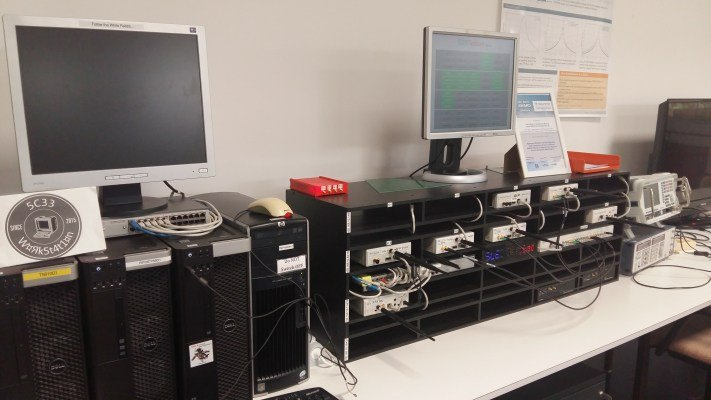
\includegraphics[width=0.70\linewidth]{SCEE_TestBed1.jpg}
    \vspace*{20pt}
    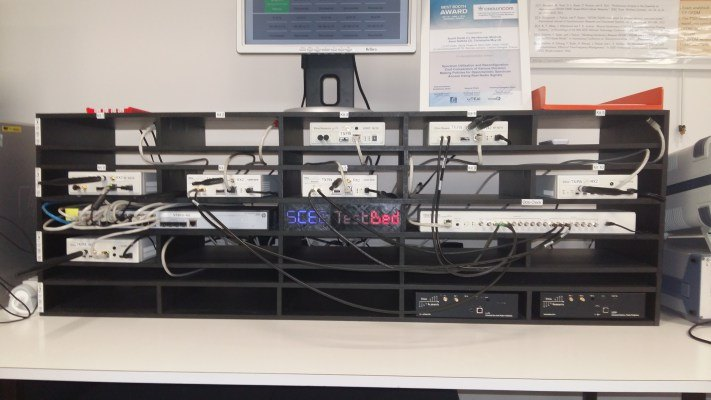
\includegraphics[width=0.70\linewidth]{SCEE_TestBed2.jpg}
    \caption{Two pictures showing the SCEE testbed \cite[Appendix~3]{Bodinier17}, taken in $2018$.}
    \label{fig:42:photosSCEETestBed}
\end{figure}

The boards have their own power supply, and are all connected to a local Ethernet switch, itself connected to a single laptop, running GNU/Linux and Ubuntu.
The pictures in Figure~\ref{fig:42:photosSCEETestBed} show the testbed used for these experiments.
% Octoclock
To ease the synchronization in both time and frequency between the boards representing the dynamic devices and the gateway, we use an Octoclock \cite{OctoclockProduct}, also a product of Ettus Research,
% https://www.ettus.com/product/details/OctoClock-G
and coaxial cables connecting every platform to the Octoclock for time (PPS) and frequency synchronization, but this is not mandatory.


\paragraph{Details about our implementation.}
%
We used the GNU Radio Companion software (GRC, version $3.7$ in $2017$),
and a laptop runs a GRC design to configure and control each USRP platform.
As such, one laptop can run in parallel the control program of any number of boards\footnote{~Even if in practice, maximum efficiency is kept as long as there is not more than one GRC design by CPU core.}.
%
The GNU Radio software provides the framework and tools to build and run software radio or just general signal-processing applications.
GNU Radio applications are flow-graphs: a series of signal processing blocks connected together to describe a data flow.
For maximum efficiency, we wrote all of our blocks in \texttt{C++}.
These flow-graphs can be written in either \texttt{C++} or the Python programming language. The GNU Radio infrastructure is written entirely in \texttt{C++}, and many of the user tools are written in Python.
GNU Radio Companion is a graphical user interface (UI) used to develop GNU Radio applications:
GRC is effectively a Python code-generation tool.
When a flow-graph is compiled in GRC, a Python code is produced, which can be executed to connect to the USRP,
create the desired GUI windows and widgets, and create and connect the blocks in the flow-graph.

Illustrations of the flow-graph for the three components of the presented demonstration are included in Appendix~\ref{sec:4:IllustrationFlowcharts}, in Figures~\ref{fig:4app:USRP_TX_PU__v1__simple_grc}, \ref{fig:4app:USRP_RX_BTS__v1__simple_grc} and \ref{fig:4app:USRP_TX_SU__v1__simple_grc}.


\paragraph{User Interface.}

We have designed a user interface in order to visualize the results obtained  with our experimental demonstration. This user interface is shown in Figure~\ref{fig:42:UI}.
We can see that it is made of three parts, one for each USRP, as highlighted in \textcolor{darkred}{circled red numbers}.

\begin{figure}[!h]
    \centering
    \includegraphics[width=1.00\textwidth]{UI.eps}
    \caption{User interface of our demonstration.}
    \label{fig:42:UI}
\end{figure}


\begin{enumerate}[leftmargin=6mm]
    \item[(1)]
The first part is the interface of the IoT traffic generator, where we see the traffic generated by this USRP, presented in a waterfall view in the time vs frequency domain.
Messages of the random traffic, generated by surrounding static devices, are shorter in time by purpose (they could be coming from other IoT standard), in order to distinguish them from an intelligent device traffic on the ``waterfall'' visualizations of the traffic.

    \item[(2)]
The second part is the interface of the intelligent device which is made of four parts.
At the top left, we observe the constellation of the transmitted packet \emph{(a)}.
At the bottom left, we have a time/frequency view of the lasts packets transmitted by the device \emph{(b)}.
We can see, in this view that the device transmitted its last $9$ packets in channels $\#3$ and $\#4$.
Then, at the top right of this interface \emph{(c)}, we can see the traffic observed by this device, where we have the interfering traffic (\textcolor{darkgreen}{green}), the uplink packets transmitted by this device (\textcolor{darkred}{red}) and the acknowledgements sent by the gateway (\textcolor{darkblue}{blue}).
Colors in the ``waterfall'' represent the RF power level received at the device antenna. Hot colors are for closer elements, as for instance the device Tx antenna (reception) is close to the device Rx antenna (transmission), and consequently for the device waterfall these signals are colored in \textcolor{darkred}{red} (see graph \emph{(c)} in part (2)).
Finally, at the bottom right \emph{(d)}, we have four histograms showing the performance indicators of the chosen MAB algorithm (number of transmissions, number of successful transmissions, UCB indexes and success rates, in each channel).

    \item[(3)]
The last part is the interface of the gateway, where we can see the traffic observed by the gateway \emph{(a)} and the channels in which the last acknowledgements have been sent \emph{(b)}.
The observed traffic is coherent with \emph{(c)} of part (2), as the elements are very close the one from the others on the testbed. Colors may change, as they depend on the exact distance between the different transmitters and receivers.
\end{enumerate}


% ----------------------------------------------------------------------
\subsection{Experimental results}
\label{sub:42:results}
% ----------------------------------------------------------------------
We compare in this PoC the two algorithms described in Section~\ref{sec:2:famousMABalgorithms} (\UCB{} and Thompson sampling) against a uniform access algorithm, that uniformly selects its channel at random.
Note that we could run more algorithms, but with no real added-valued in terms of validation of the proposed learning-based approach, which is our goal.
%
For one dynamic device, three algorithms are compared by their mean successful communication rates, on a horizon of $T=2000$ communication slots, and were using three algorithms: uniform random access (in \textcolor{cyan}{cyan}), Thompson Sampling (``\textcolor{green}{TS}'', in \textcolor{green}{green}) and \UCB{} (in \textcolor{red}{red}).

\begin{figure}[!h]
	\centering
    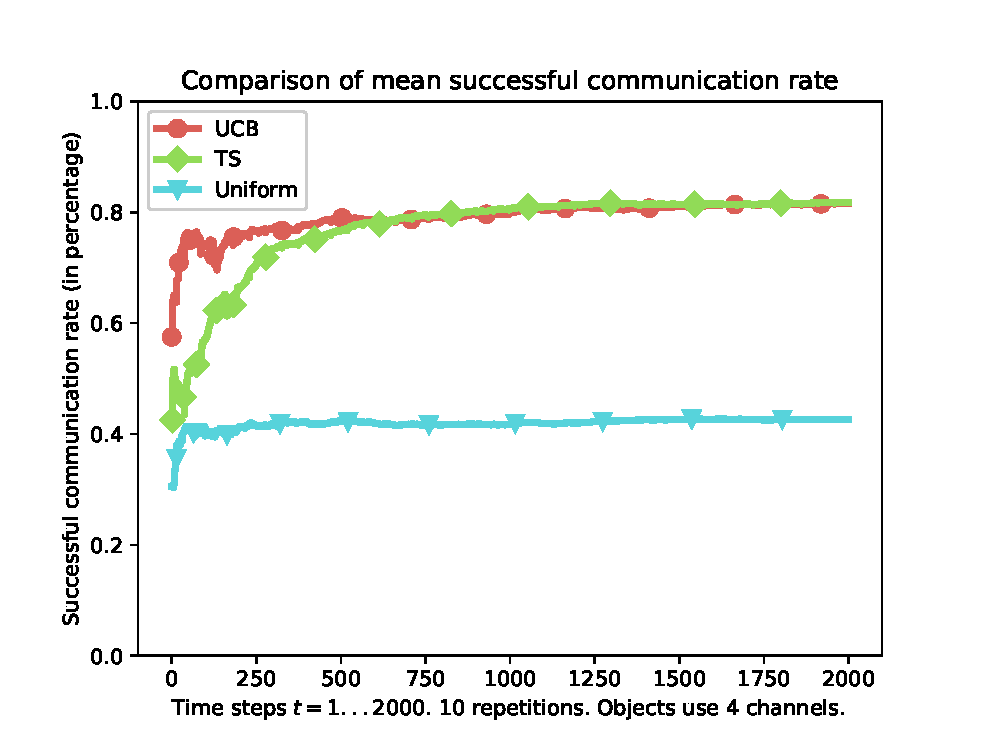
\includegraphics[height=9.0cm]{plot_datafile_append_Uniform_vs_UCB_vs_TS.eps}
    \caption{Less than $400$ communication slots (\emph{i.e.}, less than $100$ trials in each channel) are sufficient for the two learning devices to reach a successful communication rate close to $80\%$, which is \textbf{twice as much} as the non-learning (uniform) device, which stays around $40\%$ of success. Similar gains of performance were obtained in many different scenarios.}
    \label{fig:42:plot_datafile_append_Uniform_vs_UCB_vs_TS}
\end{figure}

In Figure~\ref{fig:42:plot_datafile_append_Uniform_vs_UCB_vs_TS} below, we show the results averaged on $10$ repetitions using the same conditions.
%
Each experiment has been done on a duration of about half a day,
due to the IoT sporadic transmission mode that we want to respect (like in our model of Section~\ref{sec:4:firstModel}).
However, we make devices generate one message every $5$ seconds, in order to artificially speed up the process and with no loss of generality (as we are using real hardware).
Learning can be useful only when there is a large enough difference between ``good'' and ``bad'' channels,
Each device was learning to access $4$ different non-overlapping channels, that we chose to have occupancy rates of $(\mu_k)_k = [15\%, 10\%, 2\%, 1\%]$.
Note that a maximum occupancy rate of $15\%$ could seem not so high, but indeed it is, because for a pure ALOHA access mode, a naive dynamic device only enjoys about $40\%$ success rate, under such occupancy of the channels (see the ``uniform'' plot in Figure~\ref{fig:42:plot_datafile_append_Uniform_vs_UCB_vs_TS}).
%
The occupancy rate of a channel, which denotes the mean occupancy, is implemented using the traffic generator, to emulate the presence of $S_i$ static devices with emission probability $p$ (that is, $\mu_i = S_i \times p$ here).
% They did not overlap each other, as
When facing the same stationary background traffic, we see that the learning devices are both very quickly more efficient than the naive uniform device.
We obtain an improvement in terms of successful communication rate from $40\%$ to about $60\%$ in only $100$ communications (about $16\;\mathrm{min}$), and up-to $80\%$ in only $400$ communications.
%
In stationary environments, both the TS and \UCB{} algorithms are very efficient and converge quickly, resulting in a very strong decrease in collisions and failed communication slots. \UCB{} is faster to learn but eventually TS gives a (slightly) better average performance.

Similar results are obtained for overlapping channels, when dynamic devices are learning in the presence of multiple devices, all using the same learning algorithm.
However, our experimental testbed can not run hundreds of intelligent devices.
Empirical results confirm the simulations presented in Section~\ref{sec:4:firstModel} (see Figure~\ref{fig:41:perf_learning}).
Such results are very encouraging, and illustrate well the various strong possibilities of MAB learning applied to IoT networks.

% \begin{figure}[!t]
% 	\centering
%     \begin{subfigure}[b]{0.46\textwidth}
%         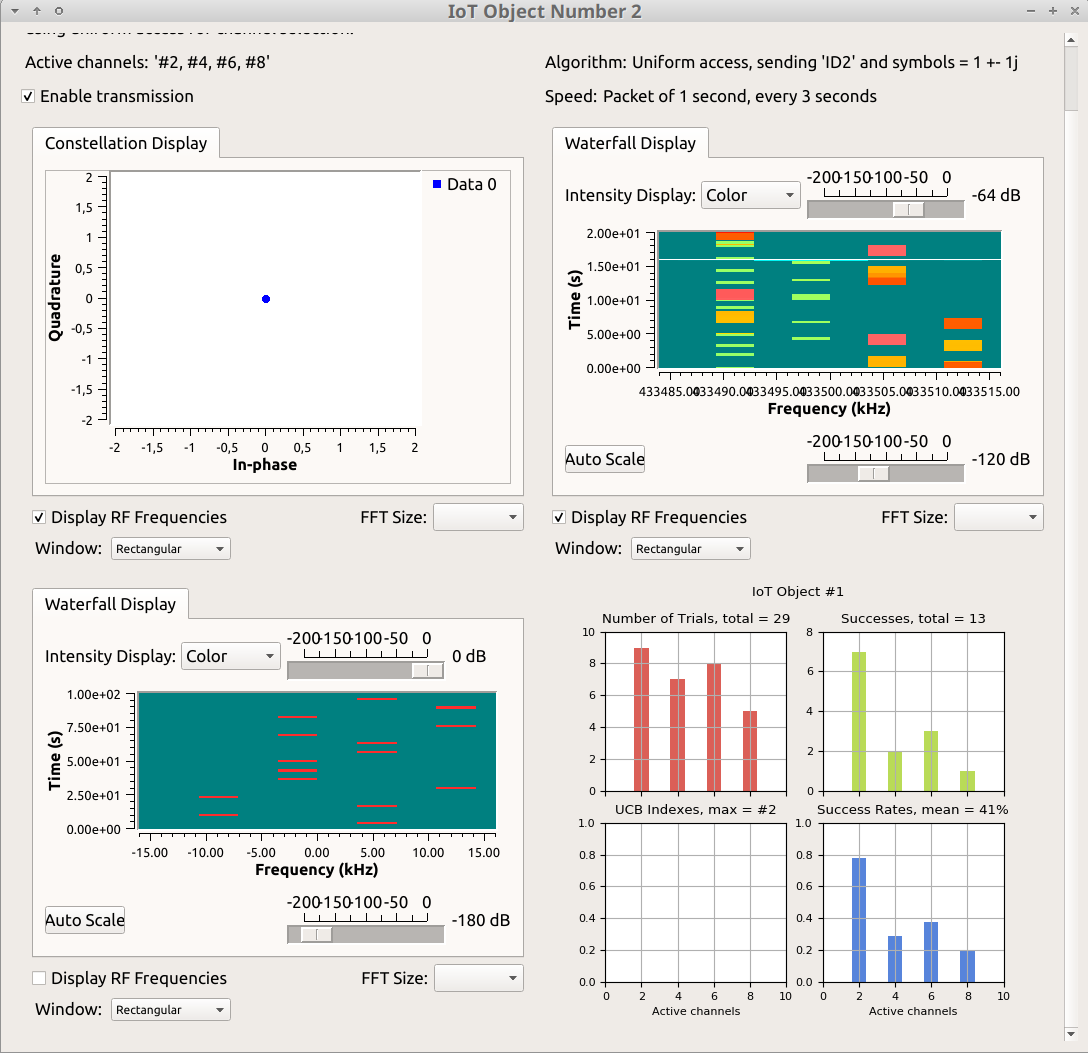
\includegraphics[height=7cm]{Object2_UniformAccess__UI.png}
%         %\caption{Device using uniform access.}
%         \label{fig:42:comparing_UniformAccess_and_UCB__1}
%     \end{subfigure}
%     ~ %add desired spacing between images, e. g. ~, \quad, \qquad, \hfill etc.
%       %(or a blank line to force the subfigure onto a new line)
%     \begin{subfigure}[b]{0.46\textwidth}
%         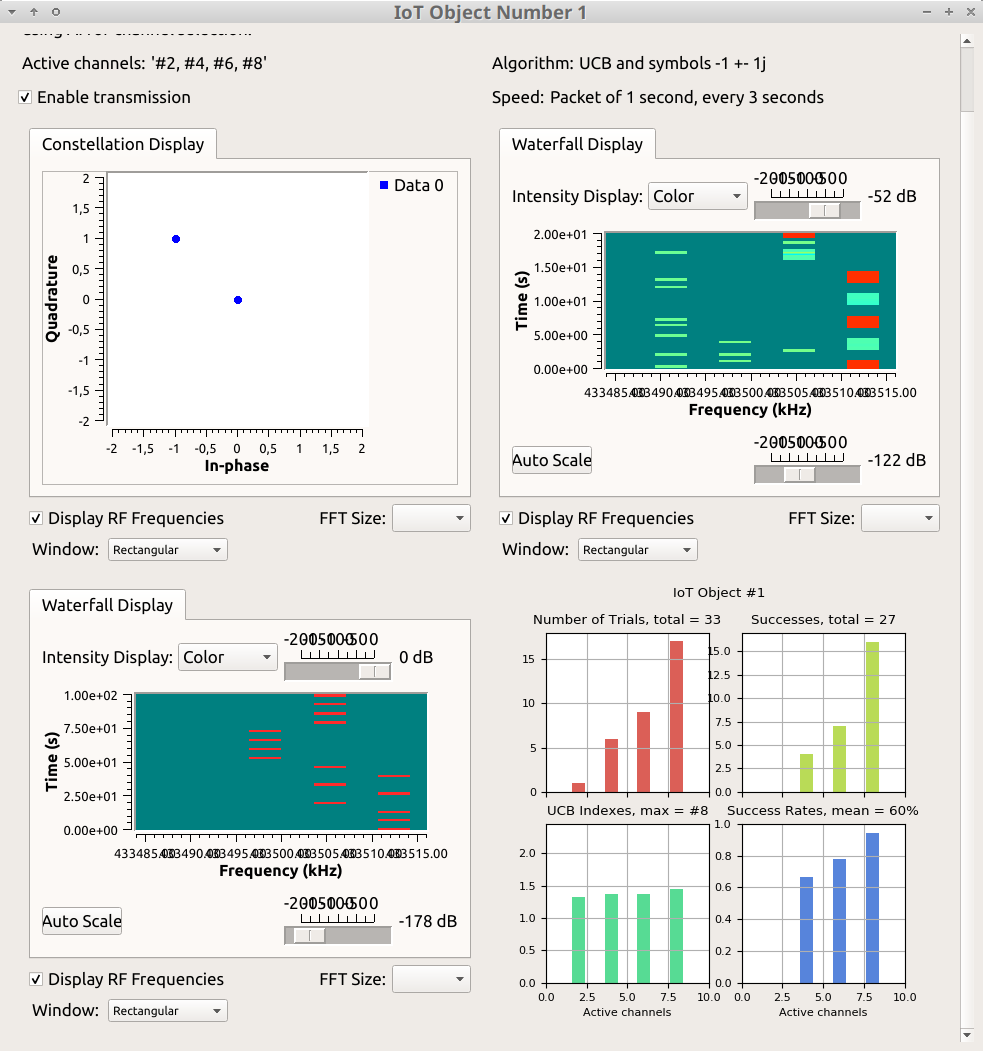
\includegraphics[height=7cm]{Object1_UCB__UI.png}
%         %\caption{Device using UCB.}
%         \label{fig:42:comparing_UniformAccess_and_UCB__2}
%     \end{subfigure}
% \caption{Comparing the success rate of an device using uniform access (left, $41\%$ of success here) and an device using the UCB algorithm (right, already $60\%$ of success). We see the learning device being much more present in the channels $\#4$ and $\#3$ (\textcolor{darkblue}{blue chart}, bottom right corner), as these channels are the less perturbed by the random interfering traffic, in this example.}
% \label{fig:42:comparing_UniformAccess_and_UCB}
% \end{figure}


\paragraph{Availability of data and materials.}
%
The source code of our demonstration is fully available online, open-sourced under GPLv3 license, at
\href{https://bitbucket.org/scee_ietr/malin-multi-arm-bandit-learning-for-iot-networks-with-grc}{\texttt{bitbucket.org/scee\_ietr/malin-multi-arm\\-bandit-learning-for-iot-networks-with-grc/}}.
%
It contains both the GNU Radio Companion flowcharts and blocks, with ready-to-use \texttt{Makefiles} to easily compile, install and launch the demonstration.
The demonstration only requires a laptop and open-source free softwares,
as the laptop should run a GNU/Linux distribution (like Ubuntu or Debian),
in addition to USRP platforms from Ettus Research.


\paragraph{Video.}
%
As depicted in Figure~\ref{fig:42:screenshotDemoYouTube} below,
we realized a $6$-minute \textbf{video} to sum-up our demonstration and advertise our work online, and it is available on the YouTube hosting platform, at \texttt{\href{https://youtu.be/HospLNQhcMk}{youtu.be/HospLNQhcMk}}.
The video shows examples of $3$ dynamic devices learning simultaneously, confirming the results of Figure~\ref{fig:42:plot_datafile_append_Uniform_vs_UCB_vs_TS} for overlapping channels.
It also shows the connections between the USRP boards, the Octoclock, the master laptop etc, completing the presentation of the SCEE testbed already shown in Figure~\ref{fig:42:photosSCEETestBed}.
% \textcolor{white}{Of course, the video was not seen much, because our work is useless! Yay!}

\begin{figure}[!h]
	\centering
    % \includegraphics[width=0.90\textwidth]{Images/screenshotDemoYouTube.png}
    \includegraphics[width=0.90\textwidth]{2-Chapters/4-Chapter/Images/screenshotDemoYouTube.png}
    \caption{Screenshot of the \textbf{video} of our demonstration, \texttt{\href{https://youtu.be/HospLNQhcMk}{youtu.be/HospLNQhcMk}}.}
    \label{fig:42:screenshotDemoYouTube}
\end{figure}

% \paragraph{Special acknowledgment.}
% %
% We acknowledge the work of two engineering students, at CentraleSup{\'e}lec campus of Rennes,
% Cl{\'e}ment Barras and Th{\'e}o Vanneuville, for their GNU Radio project in Spring $2017$,
% as we took inspiration in the GNU Radio code and the discussions we had at this time.
